\documentclass{beamer}

\usetheme{simple}

\usepackage{lmodern}
% \usepackage[scale=2]{ccicons}
\usepackage{listings}
\usepackage{graphicx}
\usepackage{hyperref}
\usepackage{xcolor}

% Go syntax highlighting
\lstdefinelanguage{Go}{
  keywords={break, default, func, interface, select, case, defer, go, map, struct,
    chan, else, goto, package, switch, const, fallthrough, if, range, type,
    continue, for, import, return, var, int, int64, string, byte, any, true, false, nil},
  keywordstyle=\color{blue}\bfseries,
  ndkeywords={make, append, len, cap, new, close, delete, copy, panic, recover, print, println},
  ndkeywordstyle=\color{teal}\bfseries,
  sensitive=true,
  comment=[l]{//},
  morecomment=[s]{/*}{*/},
  commentstyle=\color{gray}\itshape,
  stringstyle=\color{red!70!black},
  string=[b]",
  string=[b]',
  string=[b]`,
}

\lstdefinelanguage{asm}{
  keywords={MOVD, CMP, BLS, SUB, ORR, STP, ADD, JMP, BLT, CALL},
  keywordstyle=\color{blue}\bfseries,
  comment=[l]{;},
  commentstyle=\color{gray}\itshape,
  stringstyle=\color{red!70!black},
}

\lstset{
  basicstyle=\ttfamily\scriptsize,
  breaklines=true,
  frame=single,
  backgroundcolor=\color{black!5},
  numbers=none,
  tabsize=4,
  showstringspaces=false,
}

% Watermark background on every slide
\setwatermark{
\includegraphics[height=8cm]{img/Heckert_GNU_white.png}}

\title{Fear is Necessary for Optimisation}
\subtitle{A guide to writing fast, optimised Go programs}
\date{\today}
\author{Briheet Si\~ngh Yadav}
\institute{\url{https://github.com/briheet}}

\begin{document}

% ============================================================
\maketitle

% ============================================================
\begin{frame}{About Me}

  \textbf{Briheet Singh Yadav} \\
  Software Engineer --- Backend / Low Latency Systems

  \vspace{0.4cm}
  \begin{itemize}
    \item Backend \& low latency systems at work
    \item Gen-AI infra for media
    \item \textbf{Go} daily, \textbf{Rust} for fun, \textbf{C++} for competitive programming
    \item \textbf{Nix} for nix-darwin / home-manager setup. Deployments ;)
  \end{itemize}

  \vspace{0.4cm}
  \begin{block}{Find me}
    Discord: \texttt{zenin108} \quad | \quad
    X: \texttt{@brsy\_10} \quad | \quad
    GitHub: \href{https://github.com/briheet}{\texttt{briheet}}
  \end{block}

\end{frame}

% ============================================================
\begin{frame}{Overview}

  \begin{itemize}
    \item Theory + hands-on examples
    \item Tools, tricks, and ways to write \alert{better} Go code
    \item We will \alert{analyze} code and make it better step by step
    \item Find problems first, then solve them
  \end{itemize}

  \vspace{0.5cm}
  \begin{block}{Disclaimer}
    There are hundreds of optimisation tricks --- we cover the important ones here.
    Pair this with a good understanding of Go.
  \end{block}

\end{frame}

% ============================================================
\begin{frame}{Things That Bother Us}
  \framesubtitle{Why optimise at all?}

  \textbf{Latency} = delay in a system (network, I/O, heap, GC \ldots)

  \vspace{0.3cm}
  Things that bug us:
  \begin{itemize}
    \item I/O operations
    \item Synchronizations
    \item \alert{Heap allocations}
    \item \alert{GC Pressure}
  \end{itemize}

  \vspace{0.3cm}
  \textbf{Goal:} Reduce I/O overhead, reduce heap allocations, lower GC pressure.

\end{frame}

% ============================================================
\begin{frame}{A Simple Go Program}
  \framesubtitle{Where does everything happen?}

  \begin{columns}
    \column{0.45\textwidth}
    \lstinputlisting[language=Go, lastline=23]{memory/main.go}

    \column{0.55\textwidth}
    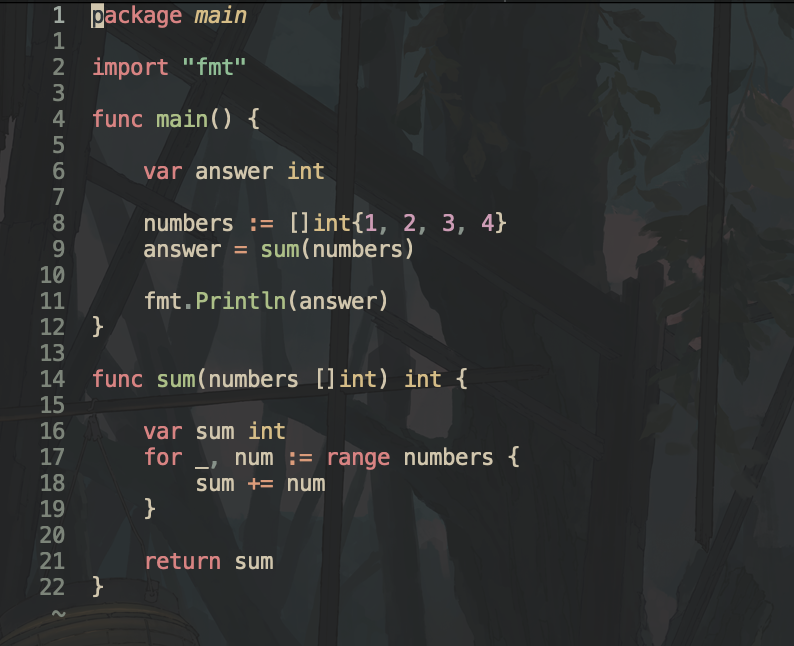
\includegraphics[width=\textwidth]{memory/short_golang_program_sum.png}
  \end{columns}

\end{frame}

% ============================================================
\begin{frame}{Reading Assembly with lensm}

  \begin{center}
    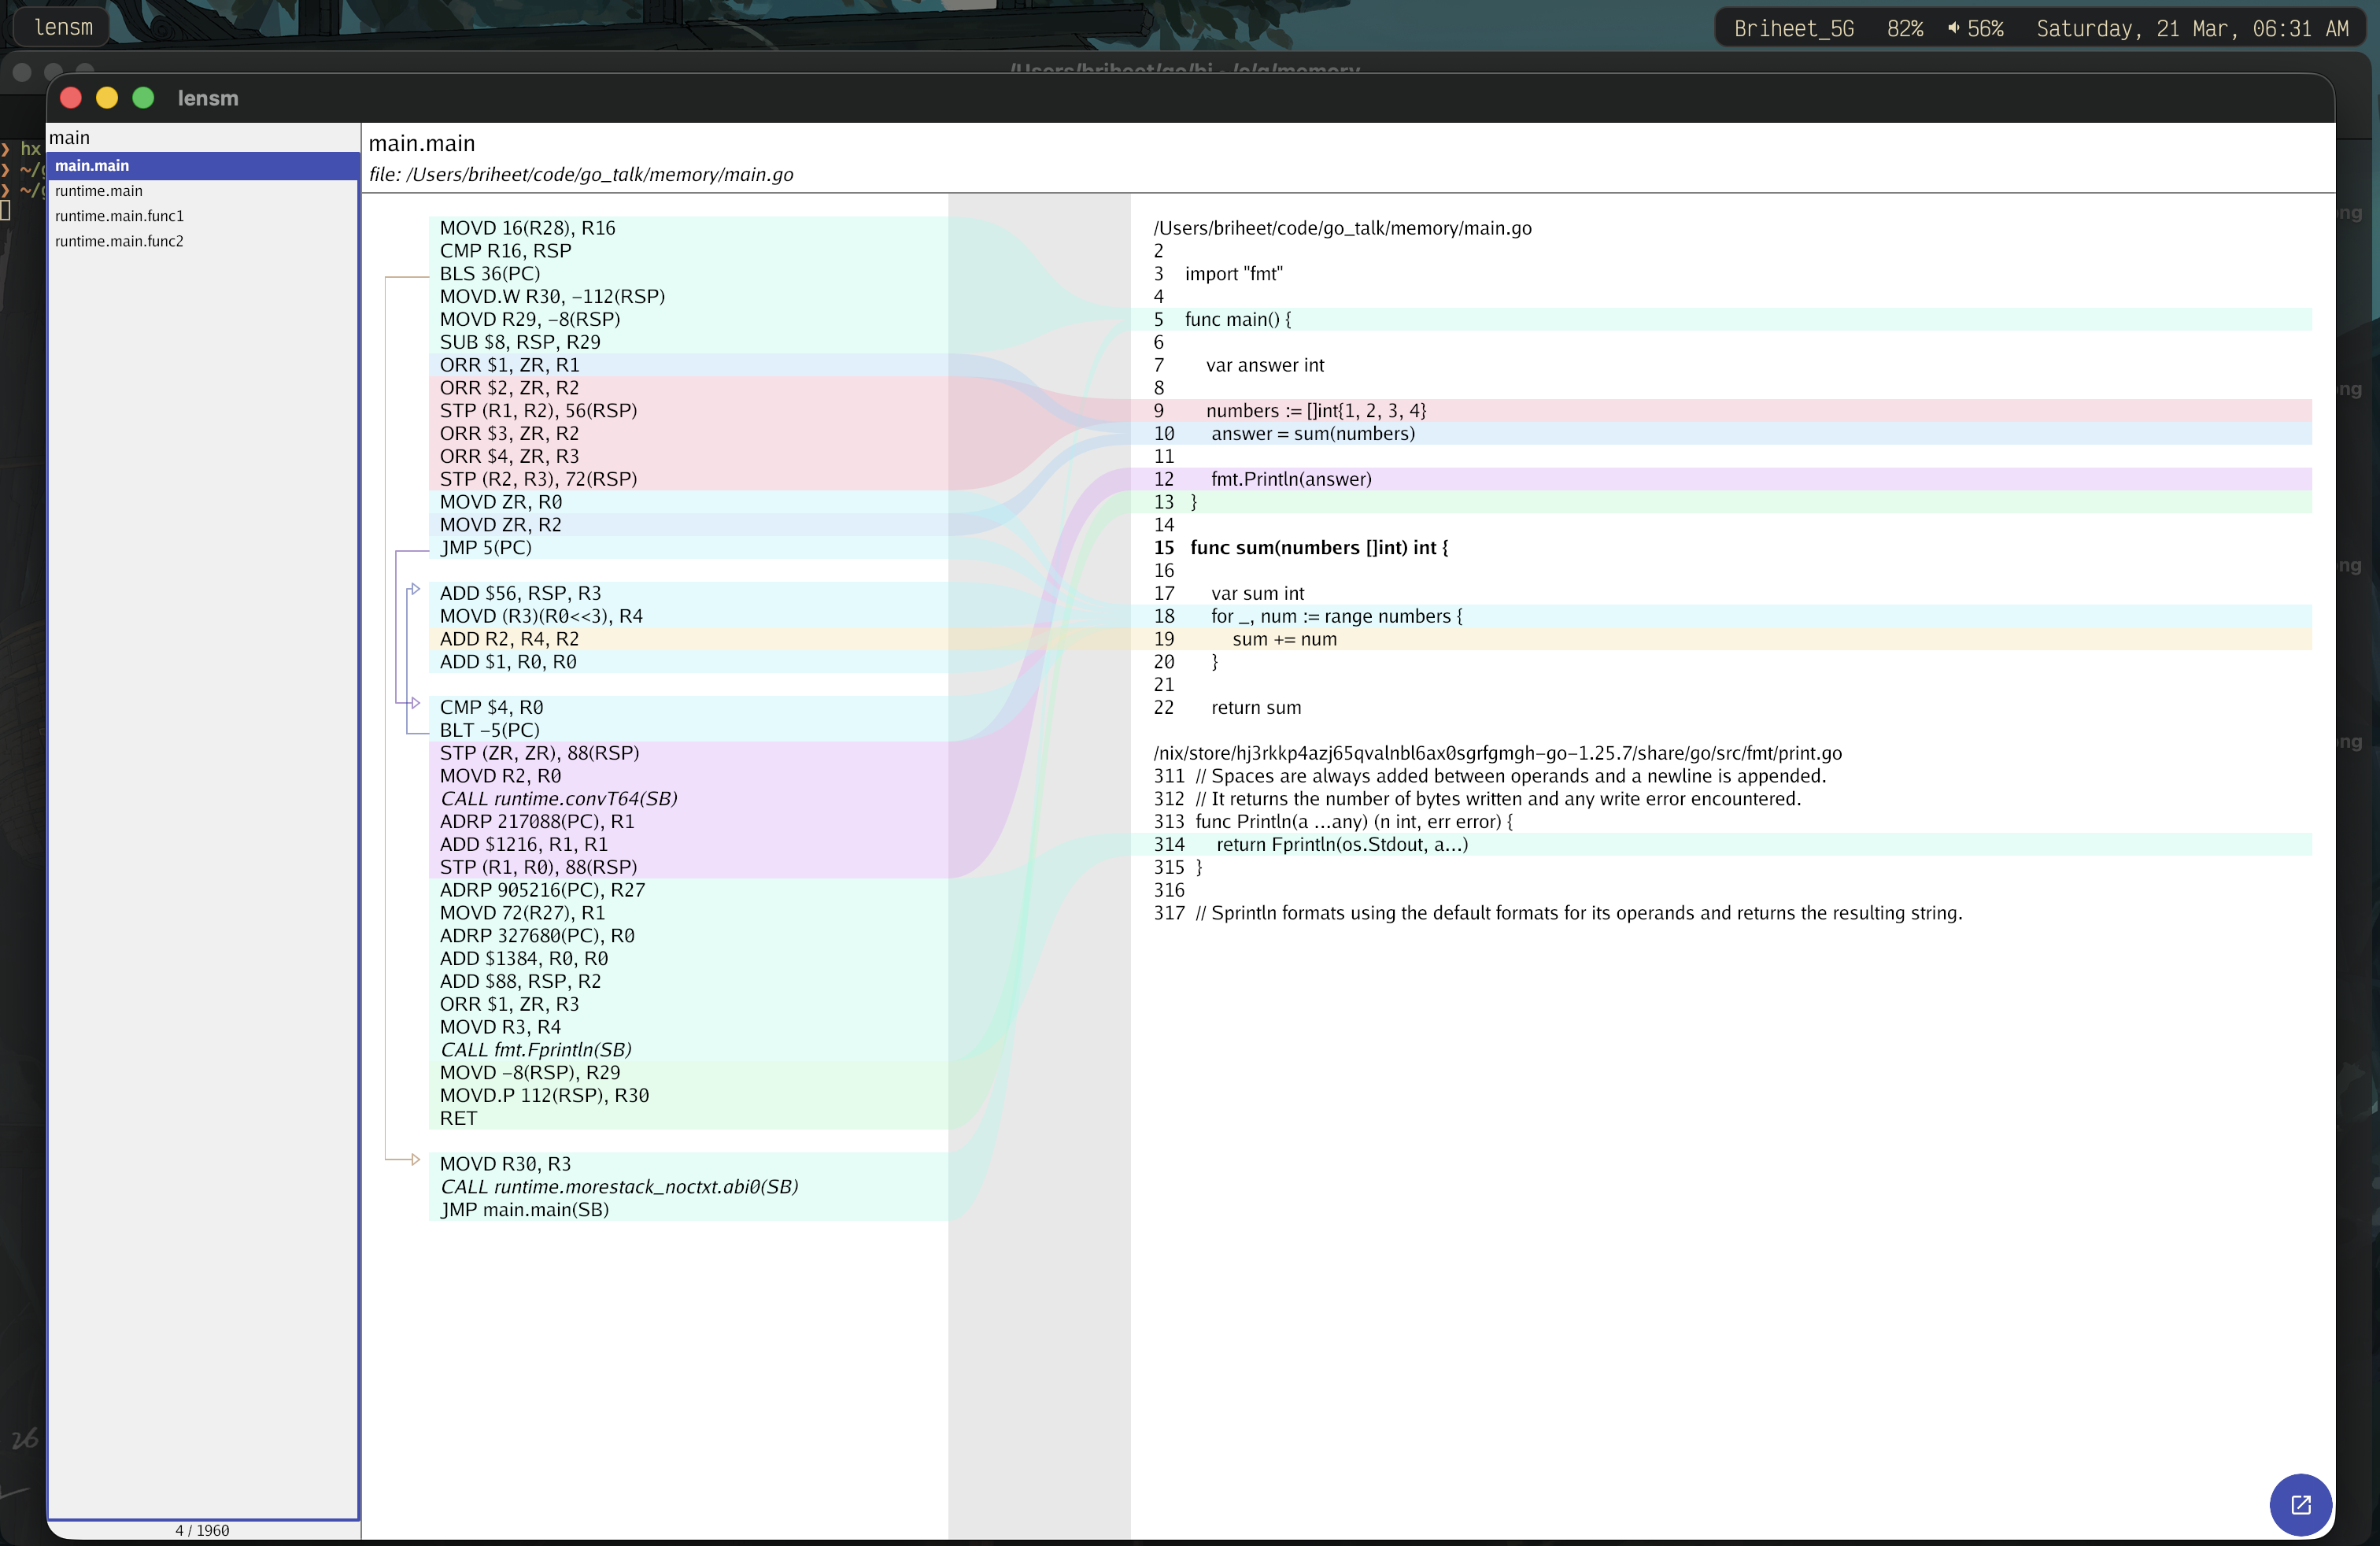
\includegraphics[width=0.85\textwidth]{memory/wholesome_lensm_output_memory.png}
  \end{center}

  \vspace{0.2cm}
  \small
  Our simple program does \emph{a lot} under the hood. \\
  Tool: \href{https://github.com/loov/lensm}{\texttt{lensm}} --- a GUI to read Go assembly.

\end{frame}

% ============================================================
\begin{frame}[fragile]{Go Assembler: MOVD}
  \framesubtitle{Go pseudo-instructions vs ARM64}

  \begin{lstlisting}[language=asm]
MOVD 16(R28), R16       ; ldr x16, [x28,#16]
  \end{lstlisting}

  \begin{columns}
    \column{0.5\textwidth}
    \small
    Go implements its own assembler pseudo-instructions for portability:
    \begin{itemize}
      \item 64-bit: \texttt{ldr, str, stur} $\Rightarrow$ \texttt{MOVD}
      \item 32-bit: \texttt{str, stur, ldrsw} $\Rightarrow$ \texttt{MOVW}
      \item 32-bit unsigned: \texttt{ldr} $\Rightarrow$ \texttt{MOVWU}
    \end{itemize}

    \column{0.5\textwidth}
    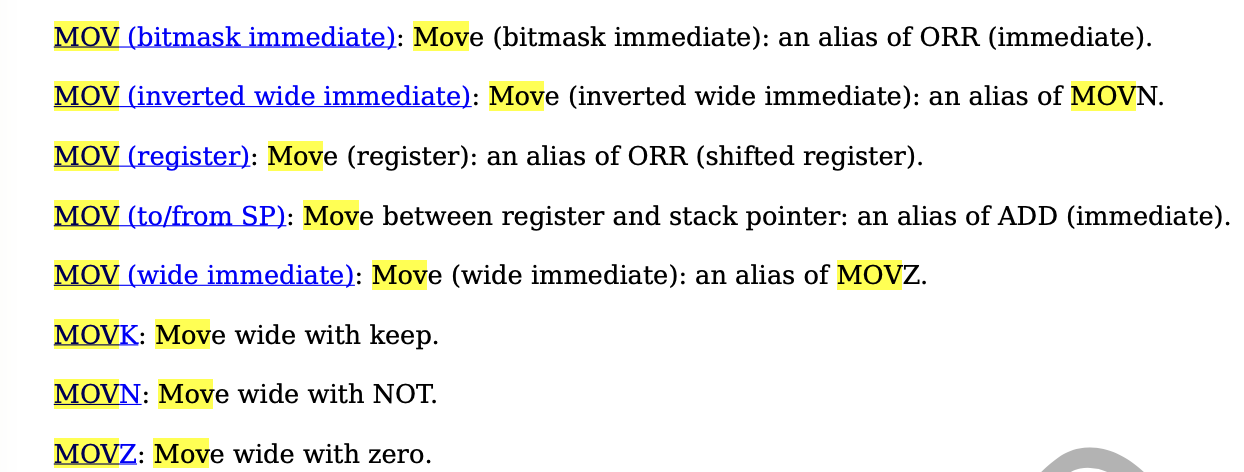
\includegraphics[width=\textwidth]{memory/core_mov_instructions.png}
  \end{columns}

  \vspace{0.2cm}
  \small
  See Rob Pike's talk: \href{https://youtu.be/KINIAgRpkDA}{Design of the Go Assembler}

\end{frame}

% ============================================================
\begin{frame}{Inside asmout: MOVD $\rightarrow$ LDR}

  \begin{columns}
    \column{0.5\textwidth}
    \centering
    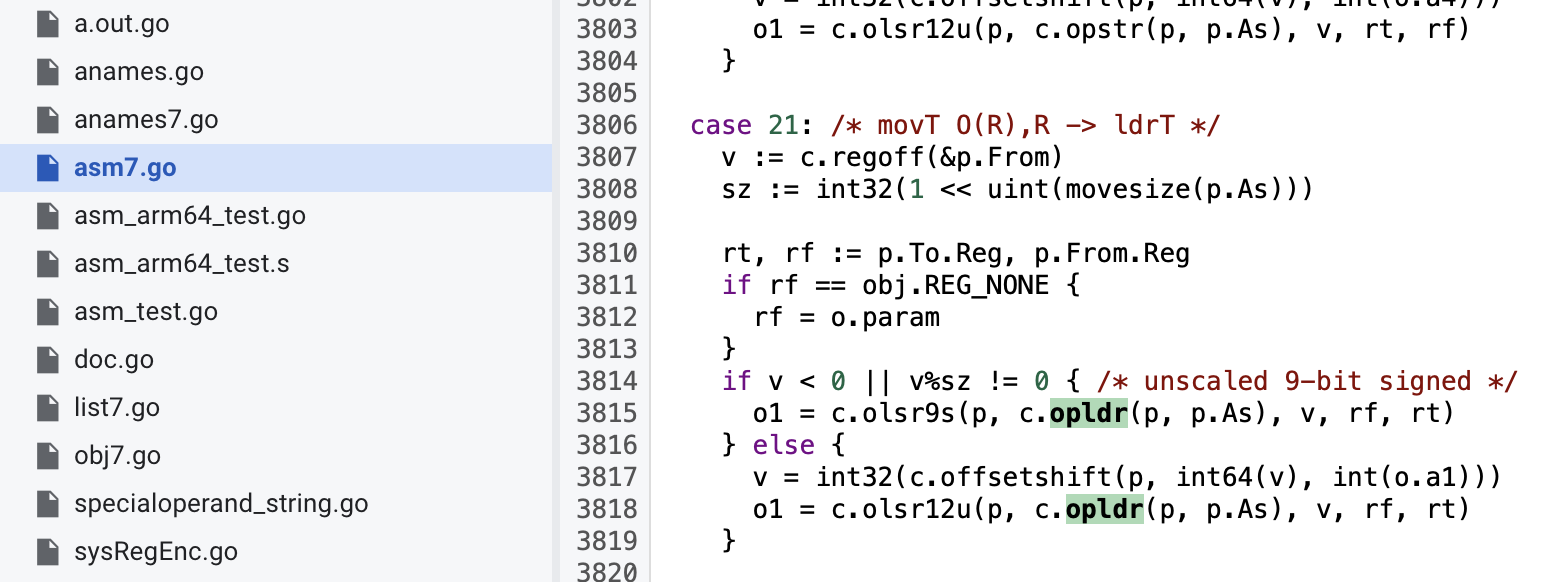
\includegraphics[width=\textwidth]{memory/movd_ldr_switch.png}
    \small Switch in \texttt{asmout}

    \column{0.5\textwidth}
    \centering
    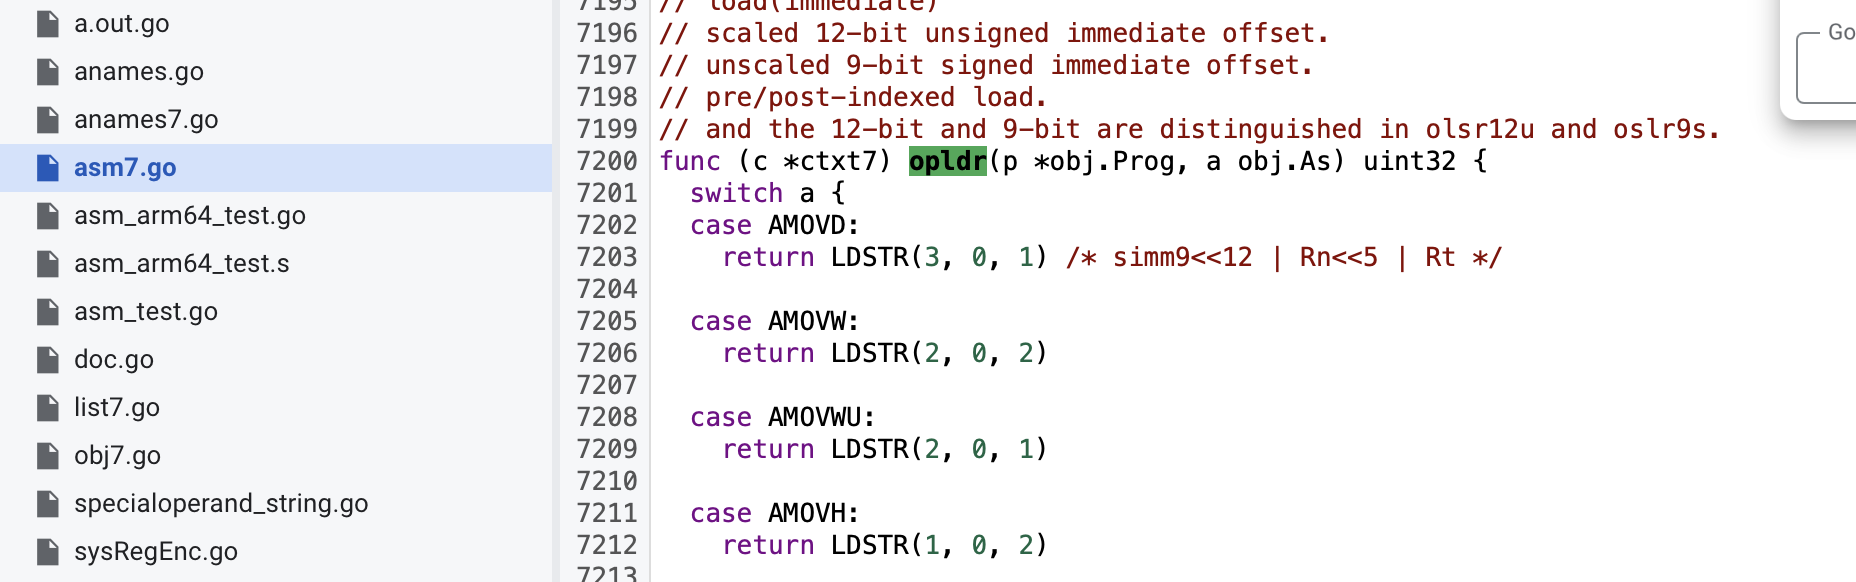
\includegraphics[width=0.95\textwidth]{memory/opldr_base_opcodes.png}
    \small Base opcodes from \texttt{opldr}
  \end{columns}

  \vspace{0.3cm}
  \begin{center}
    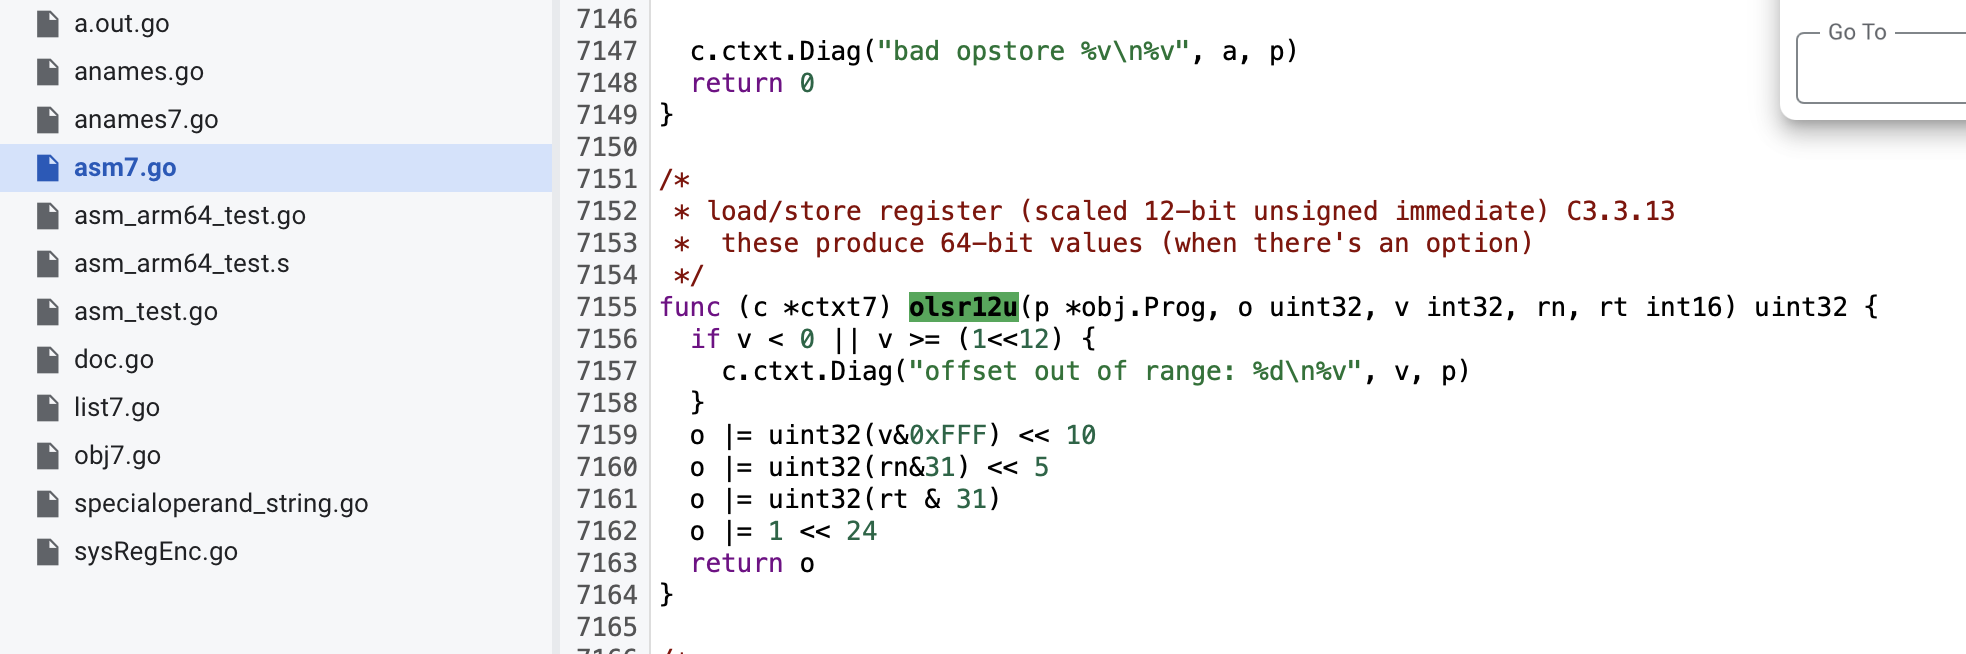
\includegraphics[width=0.45\textwidth]{memory/oslr12u.png} \\
    \small \texttt{olsr12u} encodes the immediate and sets the unsigned-offset bit.
  \end{center}

\end{frame}

% ============================================================
\begin{frame}[fragile]{R28 = Current Goroutine}
  \framesubtitle{Go ABI on ARM64}

  \begin{center}
    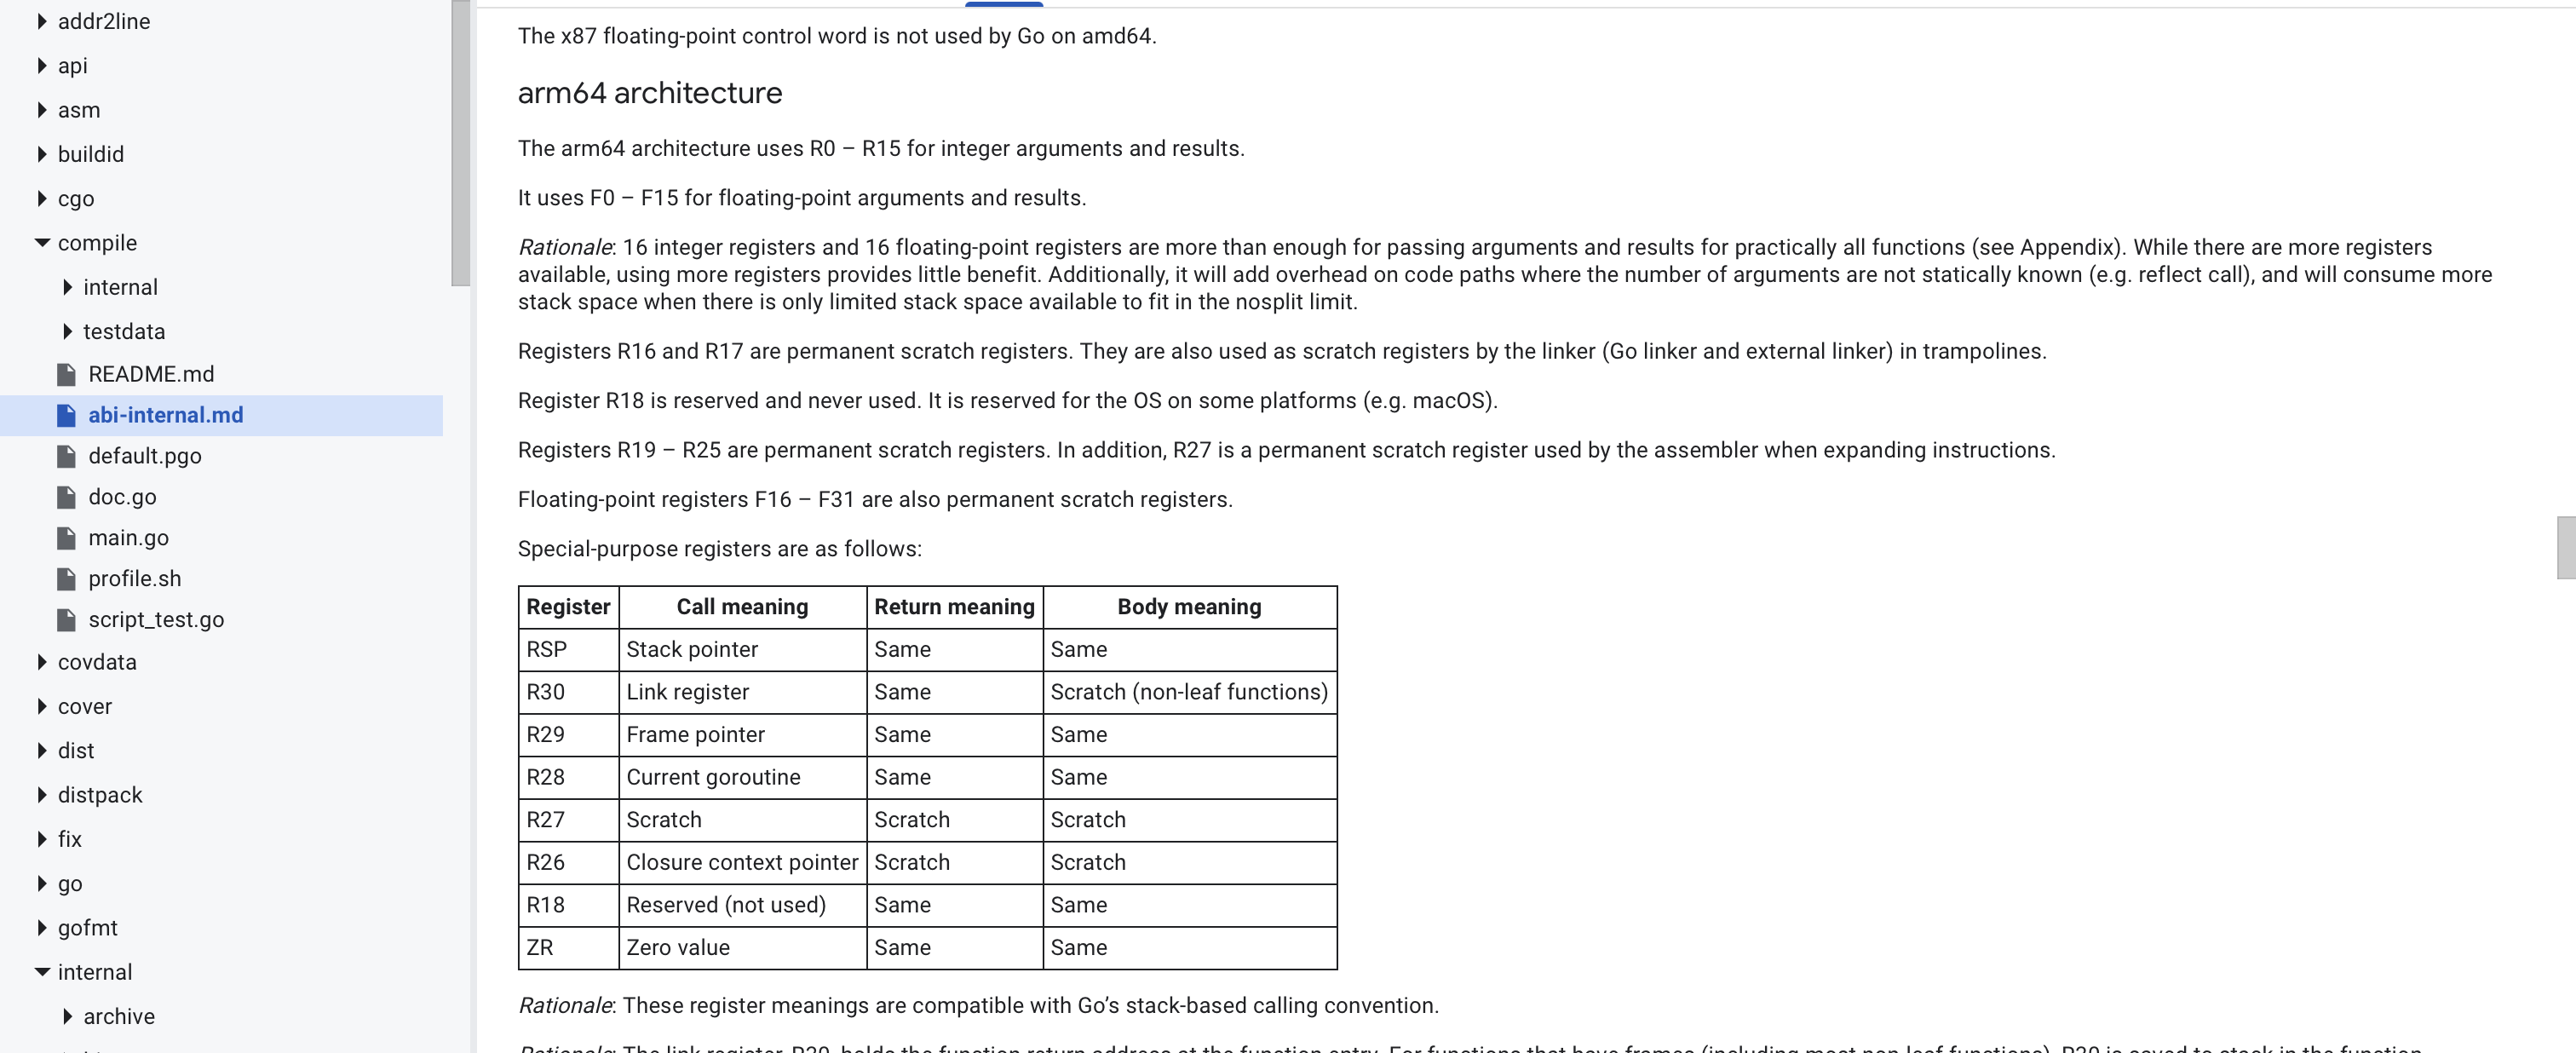
\includegraphics[width=0.7\textwidth]{memory/go_abi_arm.png}
  \end{center}

  \vspace{0.2cm}
  \begin{lstlisting}[language=asm]
MOVD 16(R28), R16       ; load g.stackguard0
CMP  R16, RSP           ; compare with stack pointer
BLS  36(PC)             ; if too close, grow stack
  \end{lstlisting}

  \small R28 is reserved by the Go compiler as the \alert{current goroutine pointer} (\texttt{g}).

\end{frame}

% ============================================================
\begin{frame}{Stack Guard \& runtime.morestack}

  \begin{center}
    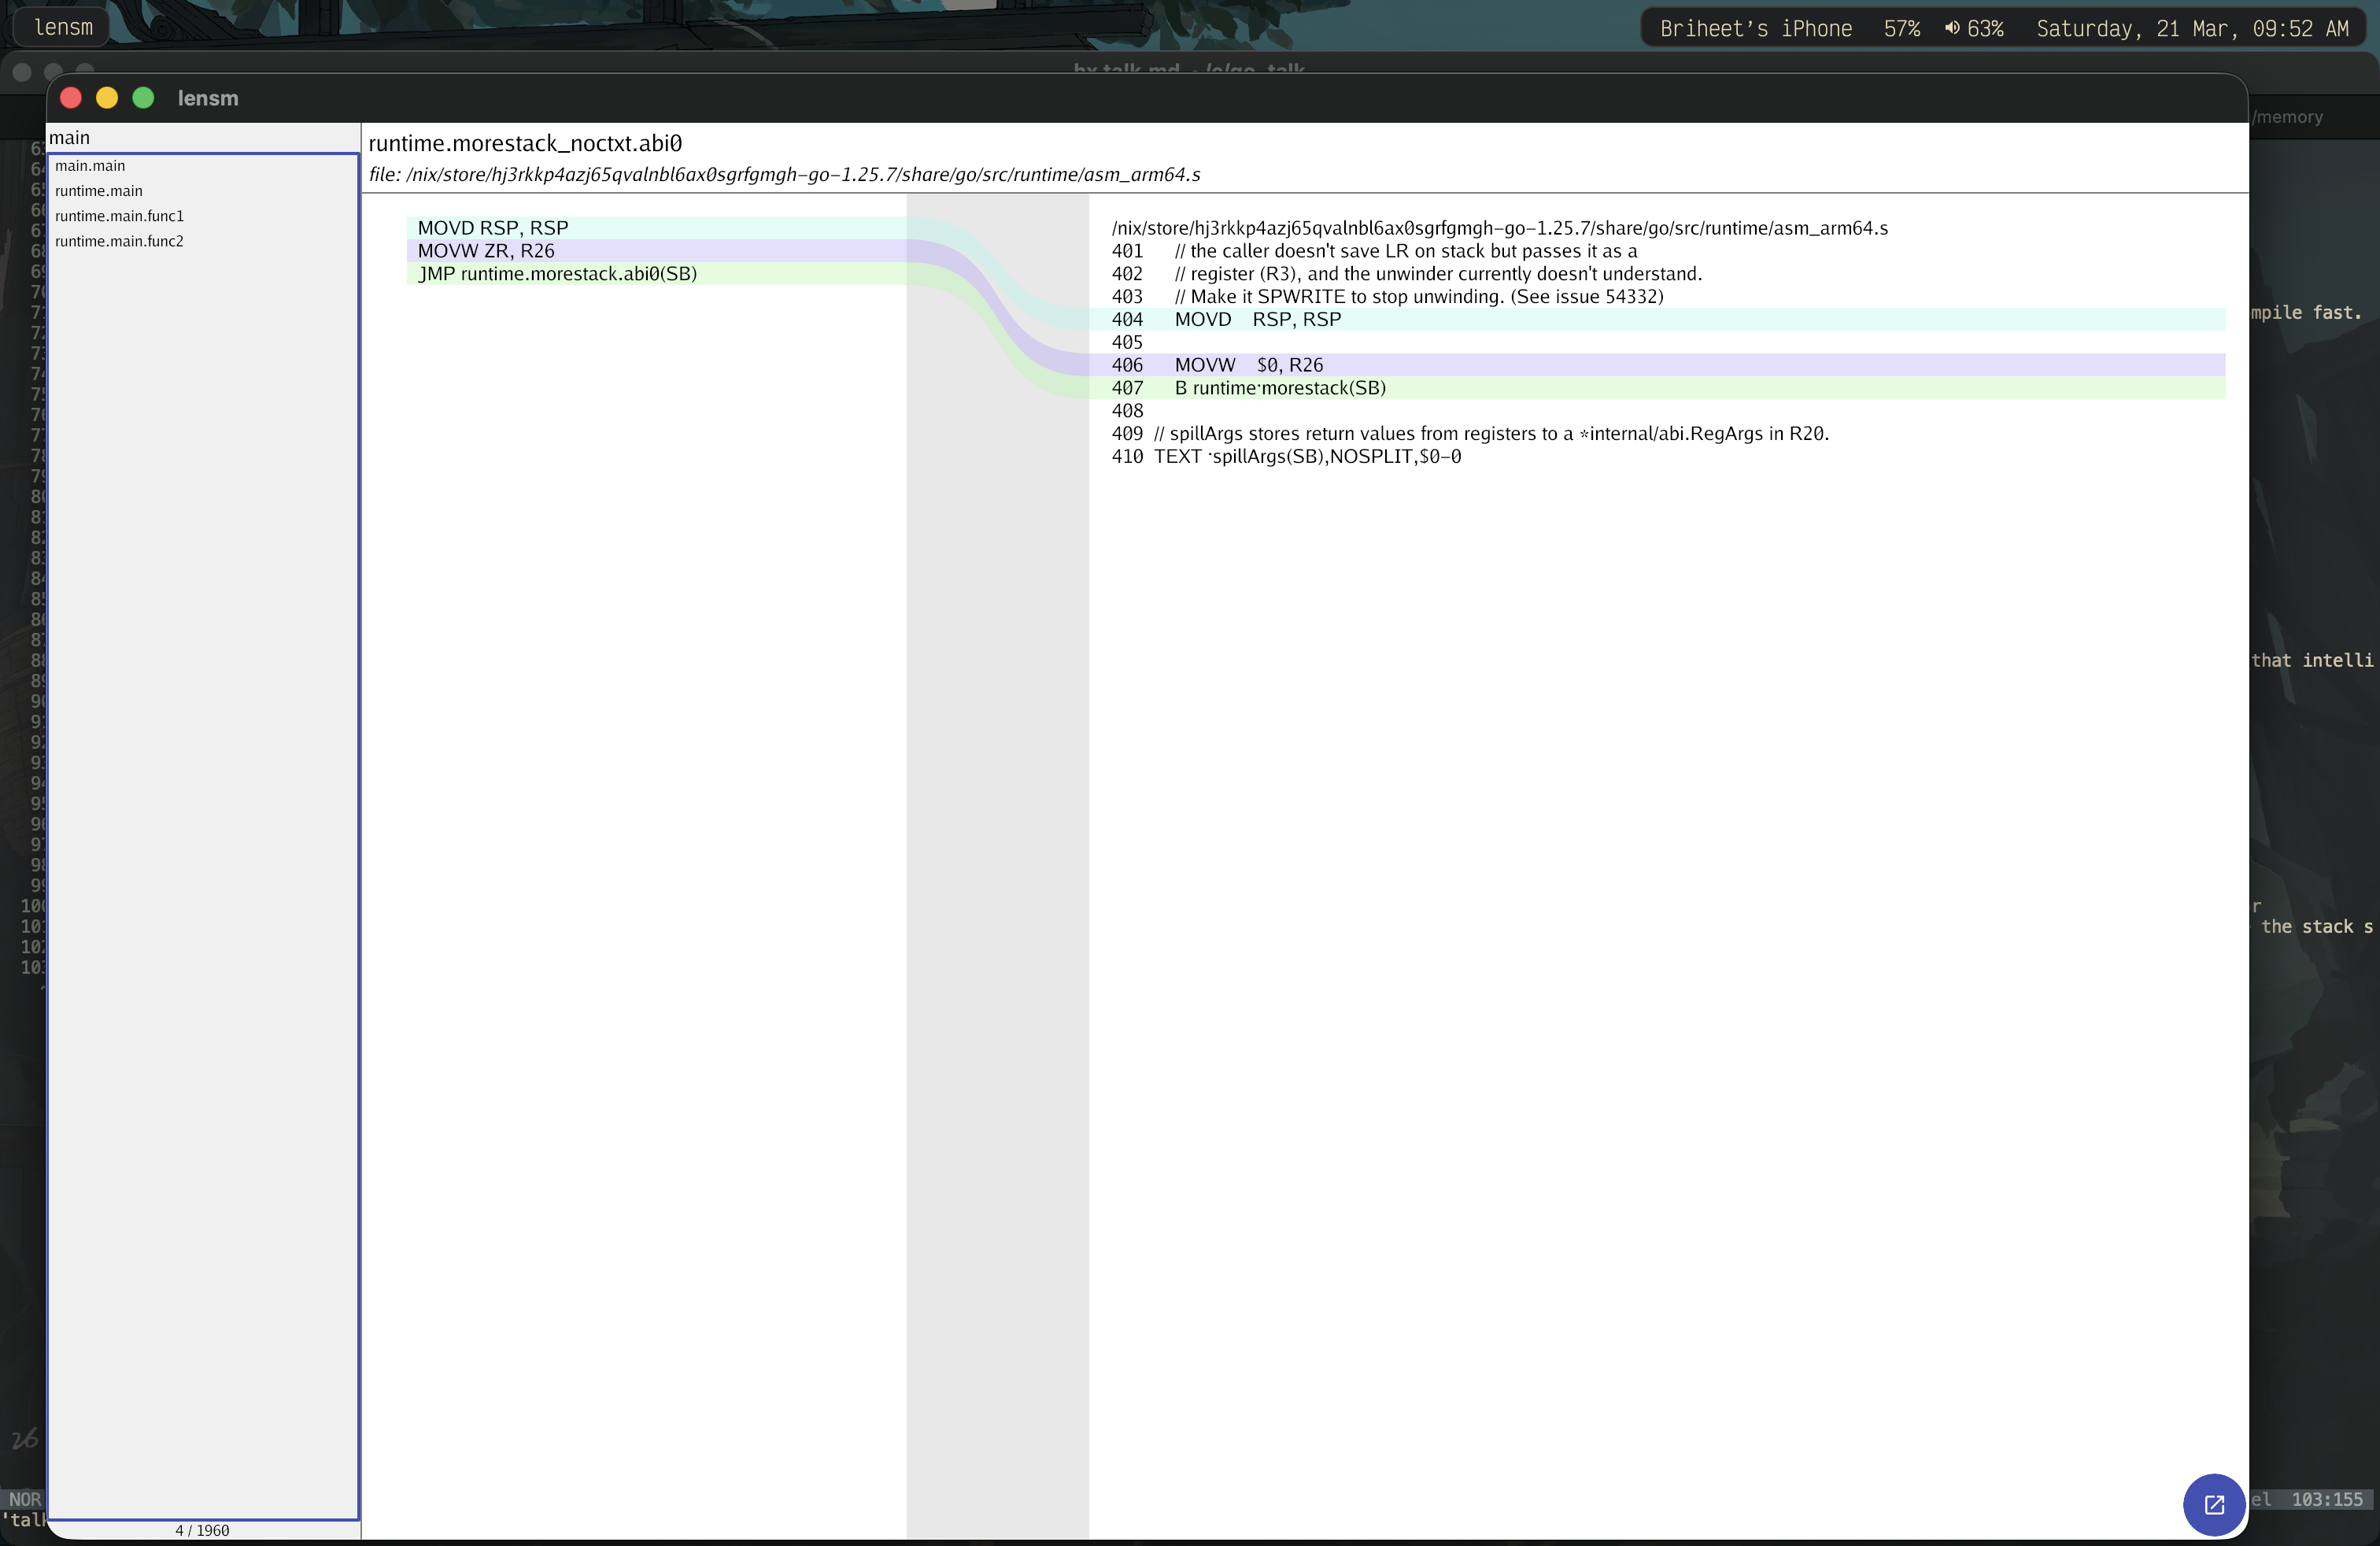
\includegraphics[width=0.75\textwidth]{memory/go_stack_increase_runtime_jump.png}
  \end{center}

  \vspace{0.3cm}
  \small
  \textbf{Flow:}
  \begin{enumerate}
    \item R28 = current goroutine (\texttt{g})
    \item \texttt{MOVD 16(R28), R16} loads \texttt{g.stackguard0}
    \item \texttt{CMP R16, SP} --- is the stack pointer too close to the guard?
    \item If yes $\rightarrow$ \texttt{runtime.morestack} grows the goroutine's stack
  \end{enumerate}

\end{frame}

% ============================================================
\begin{frame}{The Goroutine Struct (g)}

  \begin{columns}
    \column{0.55\textwidth}
    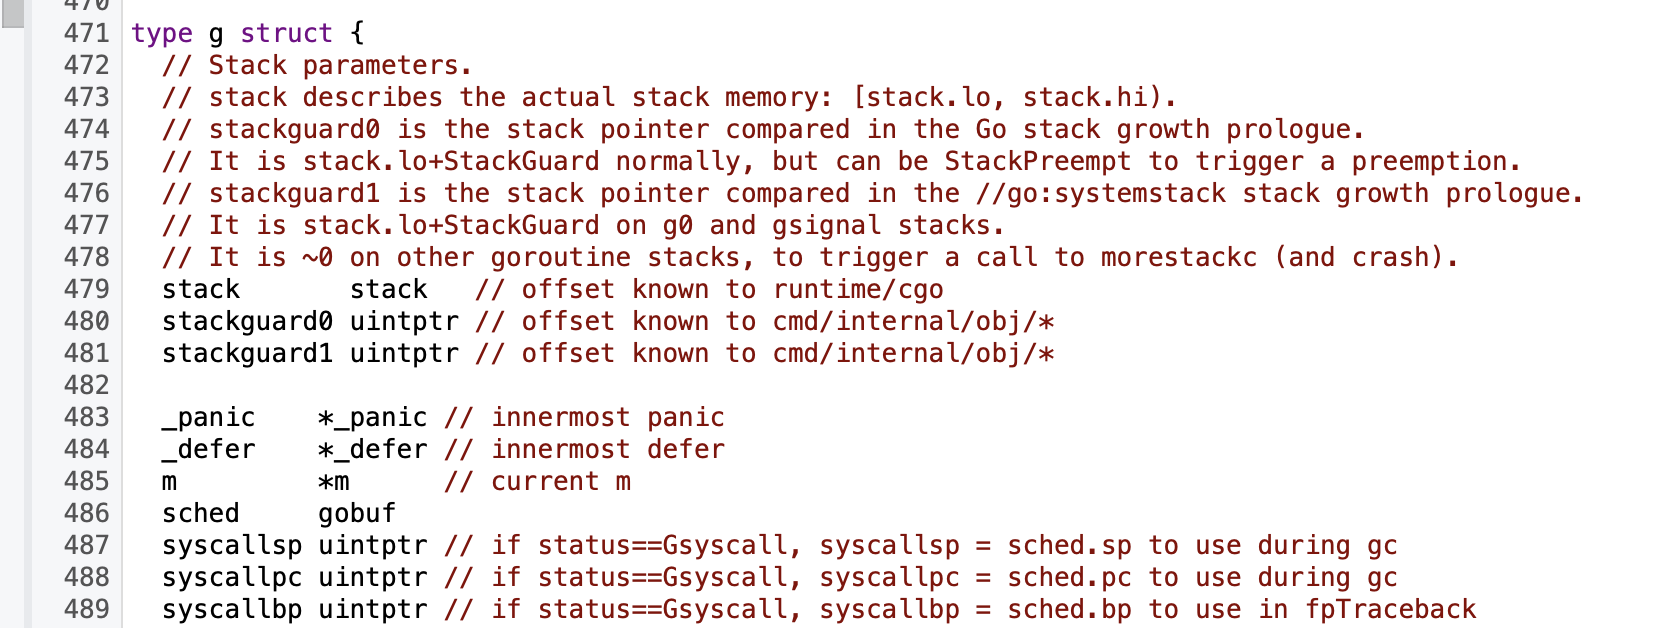
\includegraphics[width=\textwidth]{memory/g_struct.png}

    \column{0.45\textwidth}
    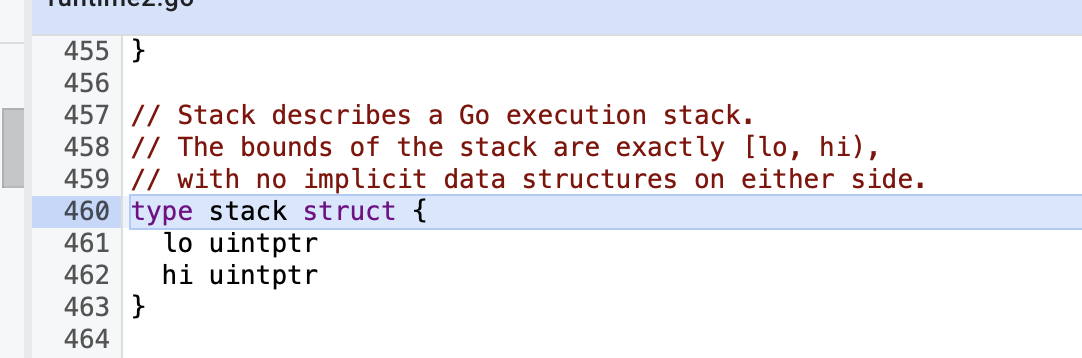
\includegraphics[width=\textwidth]{memory/lo_hi.png}

    \vspace{0.3cm}
    \small
    Offset \texttt{+0}, \texttt{+8}, \texttt{+16} \ldots \\
    \alert{+16} on R28 gives \texttt{stackguard0}.
  \end{columns}

\end{frame}

% ============================================================
\begin{frame}[fragile]{Stack Frame \& Slice Building}

  \begin{lstlisting}[language=asm]
MOVD.W R30, -112(RSP)   ; save return address
MOVD   R29, -8(RSP)     ; save frame pointer
SUB    $8, RSP, R29      ; set up frame pointer

ORR $1, ZR, R1           ; R1 = 1
ORR $2, ZR, R2           ; R2 = 2
STP (R1, R2), 56(RSP)   ; store [1,2] at SP+56
ORR $3, ZR, R2           ; R2 = 3
ORR $4, ZR, R3           ; R3 = 4
STP (R2, R3), 72(RSP)   ; store [3,4] at SP+72
  \end{lstlisting}

  \small
  Slice data lives on the stack: offsets 56--88 = 32 bytes = 4 $\times$ 8-byte ints.

\end{frame}

% ============================================================
\begin{frame}[fragile]{The Inlined Sum Loop}

  \begin{columns}
    \column{0.55\textwidth}
    \begin{lstlisting}[language=asm]
MOVD ZR, R0       ; i = 0
MOVD ZR, R2       ; sum = 0
JMP  5(PC)        ; jump to condition

ADD  $56, RSP, R3 ; base addr
MOVD (R3)(R0<<3), R4 ; load elem
ADD  R2, R4, R2   ; sum += elem
ADD  $1, R0, R0   ; i++
CMP  $4, R0       ; i < 4?
BLT  -5(PC)       ; loop back
    \end{lstlisting}

    \column{0.45\textwidth}
    \begin{lstlisting}[language=Go]
sum := 0
for i := 0; i < 4; i++ {
    sum += numbers[i]
}
    \end{lstlisting}

    \vspace{0.3cm}
    \small
    \texttt{R0<<3} = index $\times$ 8 \\
    (each \texttt{int64} is 8 bytes)

    \vspace{0.2cm}
    Jump-before-body pattern prevents executing the body before the first check.
  \end{columns}

\end{frame}

% ============================================================
\begin{frame}{The fmt.Println Trap: Interface Boxing}

  \begin{columns}
    \column{0.5\textwidth}
    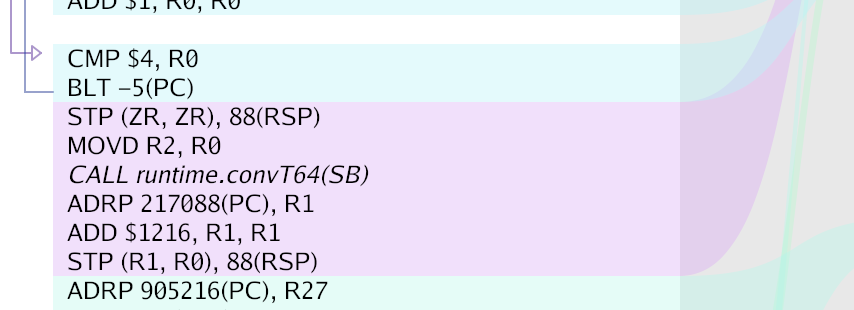
\includegraphics[width=\textwidth]{memory/runtime_call_print.png}
    \small \texttt{fmt.Println(answer)} causes \texttt{runtime.convT64}

    \column{0.5\textwidth}
    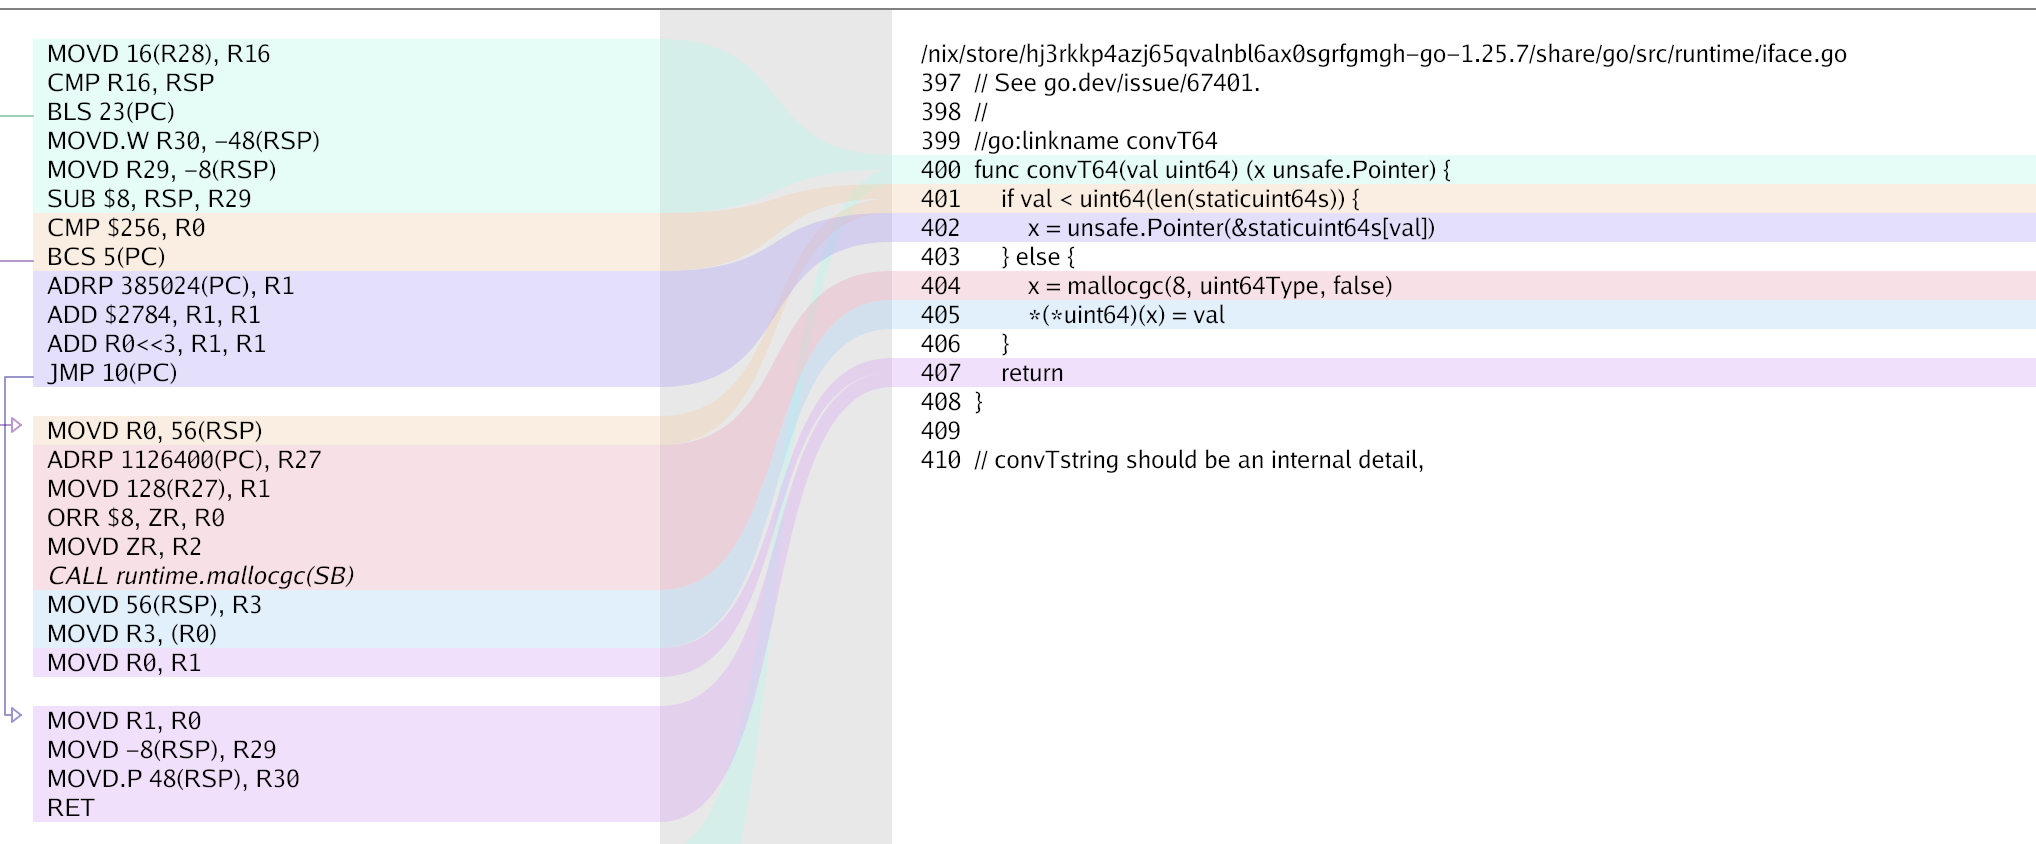
\includegraphics[width=\textwidth]{memory/convT64.png}
    \small The \texttt{convT64} implementation --- allocates at runtime!
  \end{columns}

  \vspace{0.3cm}
  \begin{block}{Why?}
    \texttt{fmt.Println(a ...any)} takes \texttt{any} (interface) --- so the value gets \alert{boxed}, causing a heap allocation.
  \end{block}

\end{frame}

% ============================================================
\begin{frame}{Part 2: CPU Profiling}
  \framesubtitle{Measure, don't guess}

  \begin{center}
    {\Large \textbf{CPU Profiling}} \\
    \vspace{0.3cm}
    Measuring where your program spends CPU time. \\
    Records which functions consume the most cycles.
  \end{center}

  \vspace{0.5cm}
  \begin{block}{Tools}
    \texttt{go test -bench}, \texttt{pprof}, \texttt{benchstat}, \texttt{lensm}
  \end{block}

\end{frame}

% ============================================================
\begin{frame}[fragile]{The Victim Program}

  \begin{lstlisting}[language=Go]
func calculateResult(num int) string {
    var result string
    for i := range num {
        result += fmt.Sprintf("item-%d,", i)
    }
    return result
}
  \end{lstlisting}

  \begin{lstlisting}[language=bash]
$ go run main.go
elapsed: 2.649227084s
length: 100101
  \end{lstlisting}

  \alert{2.6 seconds} for string building. Yikes.

\end{frame}

% ============================================================
\begin{frame}{Writing Tests \& Benchmarks}

  \begin{columns}
    \column{0.5\textwidth}
    \centering
    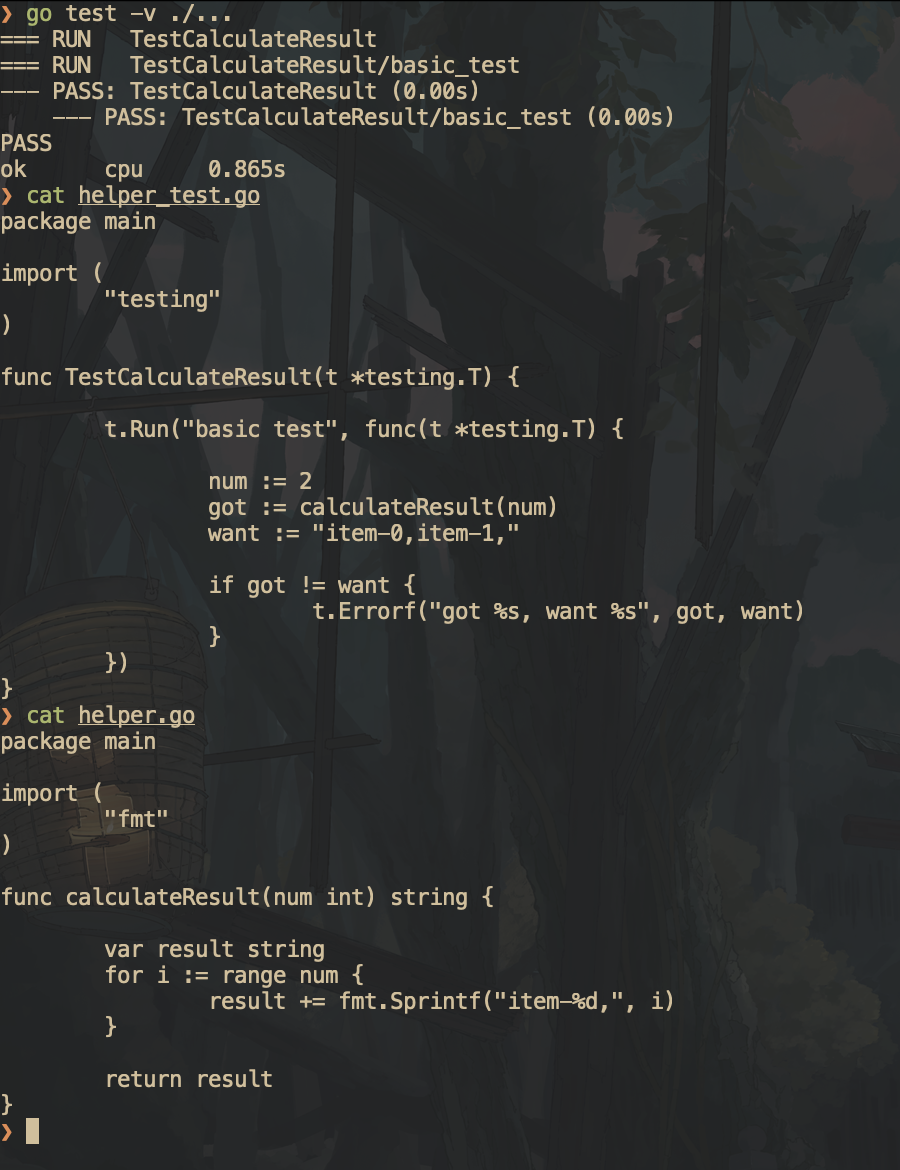
\includegraphics[width=0.95\textwidth]{cpu/test.png} \\
    \small Test passes

    \column{0.5\textwidth}
    \centering
    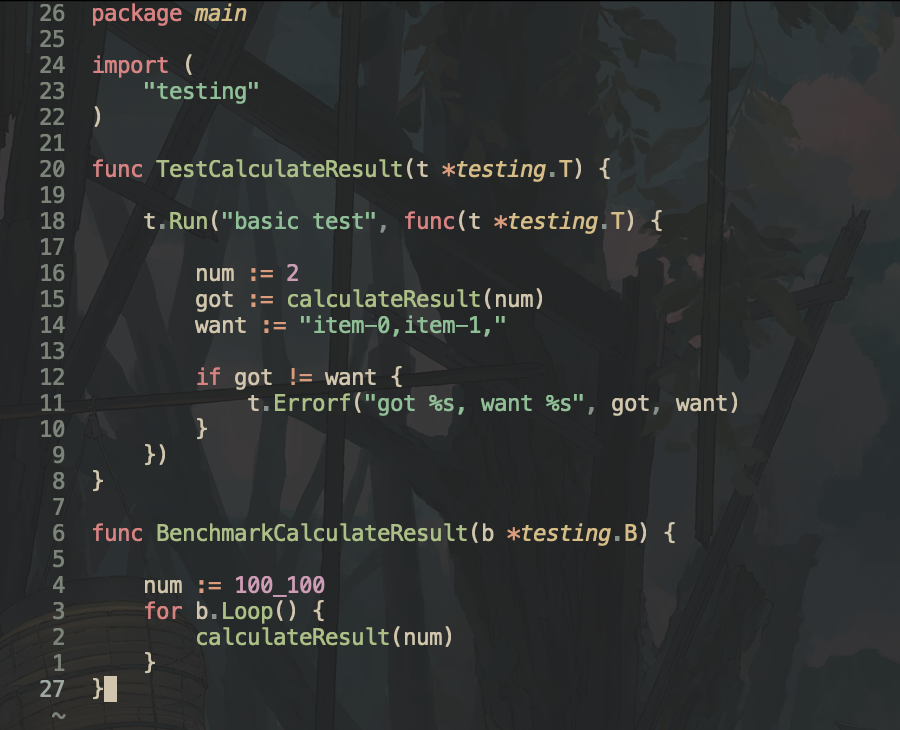
\includegraphics[width=0.95\textwidth]{cpu/benchmark.png} \\
    \small Benchmark setup
  \end{columns}

  \vspace{0.3cm}
  \small
  Always write tests first so optimisations don't break correctness.

\end{frame}

% ============================================================
\begin{frame}[fragile]{Benchmarking Flags}

  \begin{lstlisting}[language=bash]
go test -bench=. -benchmem -benchtime=3s \
  -count=10 -cpuprofile=cpu.pprof \
  -memprofile=mem.pprof > benchmark.txt
  \end{lstlisting}

  \vspace{0.2cm}
  \small
  \begin{itemize}
    \item \texttt{-bench=.} --- run all benchmarks
    \item \texttt{-benchmem} --- include memory allocation stats
    \item \texttt{-benchtime=3s} --- each benchmark runs for 3 seconds
    \item \texttt{-count=10} --- repeat 10 times (profilers are non-deterministic)
    \item \texttt{-cpuprofile} / \texttt{-memprofile} --- save profiles for pprof
  \end{itemize}

\end{frame}

% ============================================================
\begin{frame}[fragile]{Baseline: The Ugly Numbers}

  \begin{lstlisting}[language=bash]
BenchmarkCalculateResult-12   2  2545ms  54GB/op  329k allocs/op
  \end{lstlisting}

  \begin{center}
    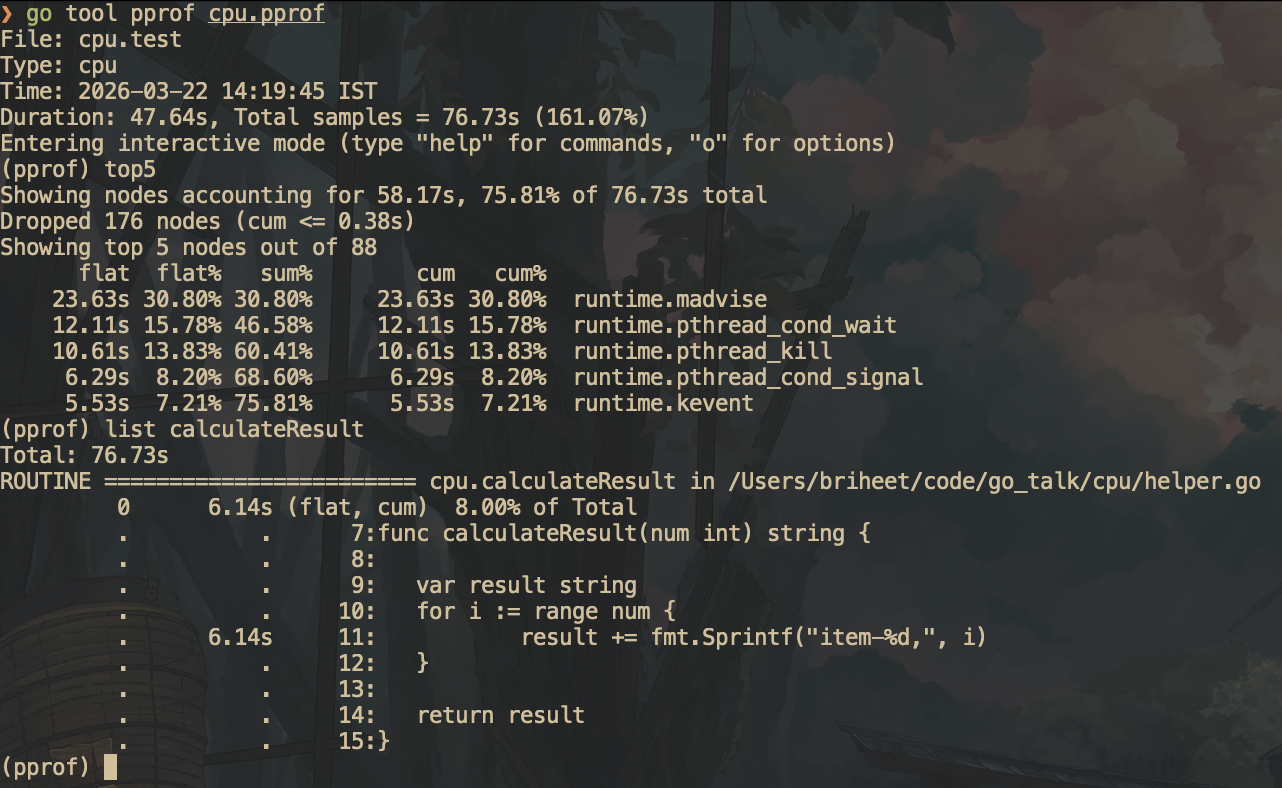
\includegraphics[width=0.7\textwidth]{cpu/cpu_pprof.png}
  \end{center}

  \small
  pprof shows \alert{6 seconds} on the result line --- and that's only 8\% of the program!

\end{frame}

% ============================================================
\begin{frame}[fragile]{Profiling Reveals: Memory is the Bottleneck}

  \begin{lstlisting}[language=bash]
(pprof) list calculateResult
Total: 912.98GB
  912.70GB  912.97GB  11: result += fmt.Sprintf("item-%d,", i)
  \end{lstlisting}

  \vspace{0.3cm}
  \small
  \texttt{fmt.Sprintf} itself is only 170ms --- the real problem is \alert{string concatenation}:
  \begin{enumerate}
    \item \texttt{runtime.convT64} --- interface boxing for \texttt{...any}
    \item \texttt{runtime.concatstring2} --- the \texttt{result +=} copies the entire string each time $\Rightarrow$ \alert{O(n\textsuperscript{2})}
  \end{enumerate}

\end{frame}

% ============================================================
\begin{frame}[fragile]{Fix \#1: strings.Builder}

  \begin{columns}
    \column{0.5\textwidth}
    \begin{lstlisting}[language=Go]
func calculateResult(num int) string {
    var sb strings.Builder
    for i := range num {
        sb.WriteString(
            fmt.Sprintf("item-%d,", i))
    }
    return sb.String()
}
    \end{lstlisting}

    \column{0.5\textwidth}
    \begin{lstlisting}[language=bash]
$ go run .
elapsed: 11.362125ms
    \end{lstlisting}

    \vspace{0.3cm}
    \small
    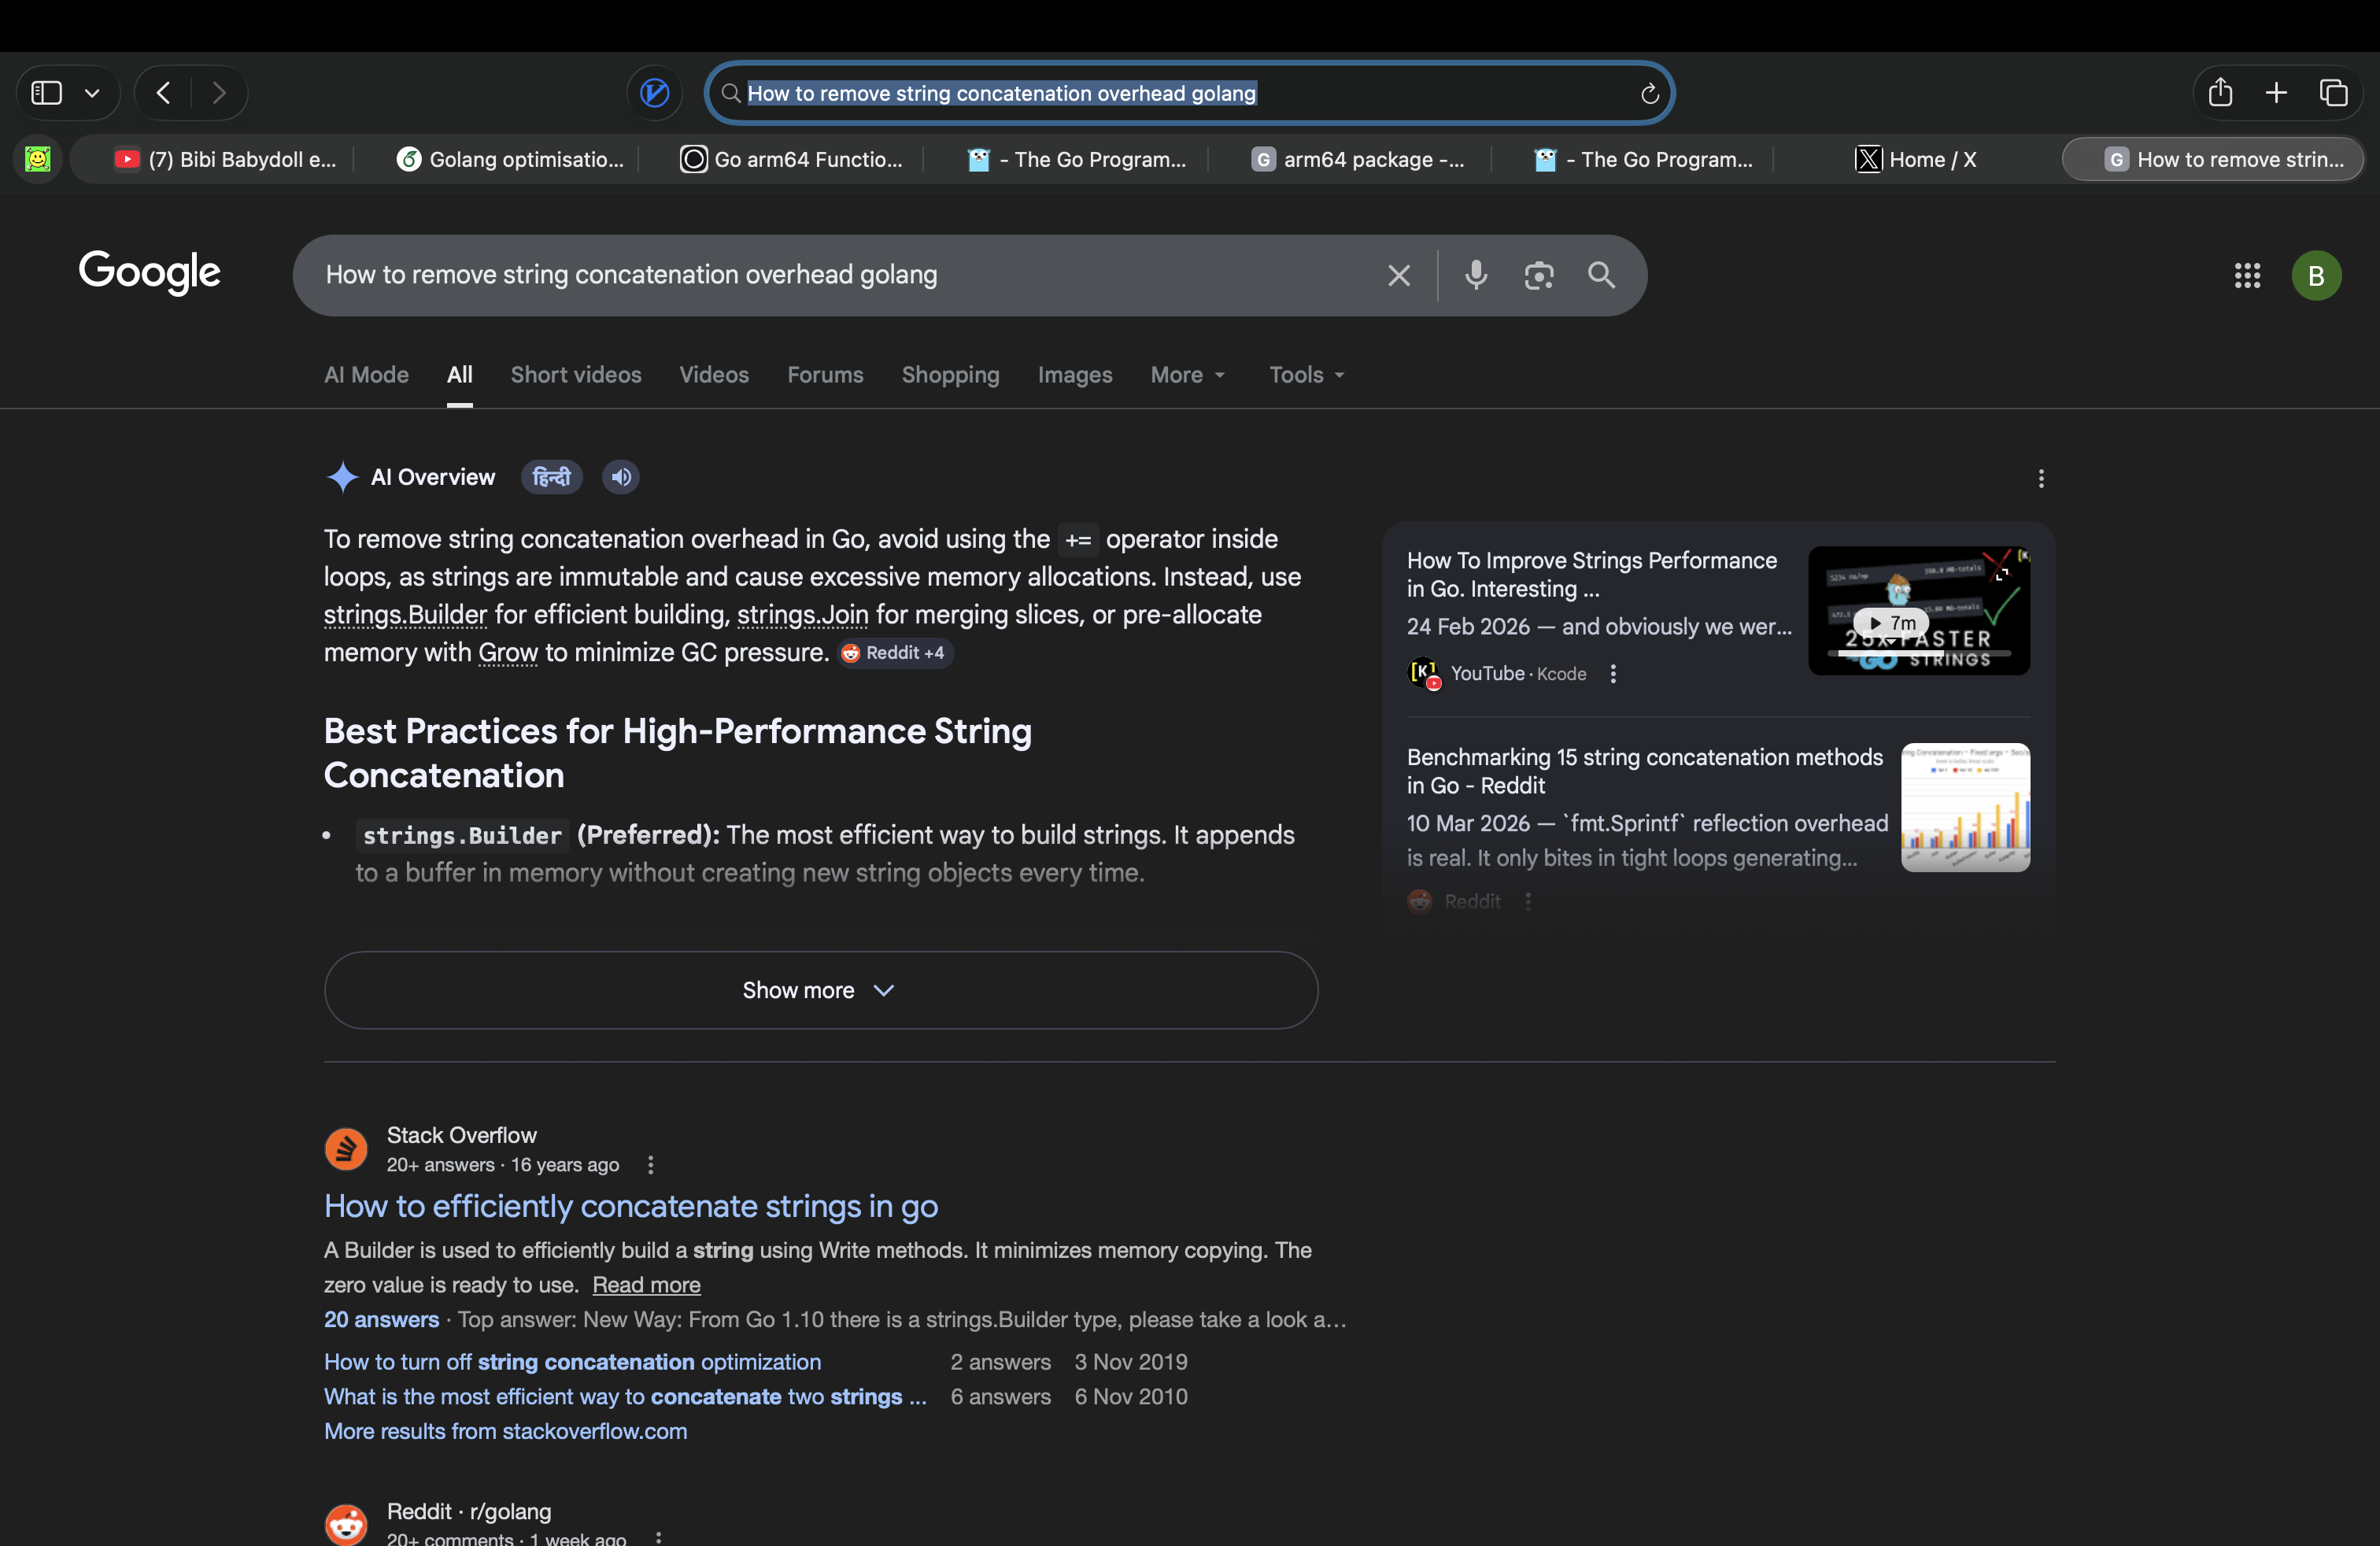
\includegraphics[width=\textwidth]{cpu/google_result.png}
  \end{columns}

  \vspace{0.3cm}
  \begin{block}{benchstat: v0 vs v1}
    Time: 2545ms $\rightarrow$ 4.5ms (\alert{-99.82\%}) \\
    Memory: 52 GB $\rightarrow$ 7 MB (\alert{-99.99\%}) \\
    Allocs: 330k $\rightarrow$ 200k (\alert{-39\%})
  \end{block}

\end{frame}

% ============================================================
\begin{frame}[fragile]{Fix \#2: Drop fmt.Sprintf}

  \begin{lstlisting}[language=Go]
var itemBytes = []byte{0x69, 0x74, 0x65, 0x6d, 0x2d} // "item-"

func calculateResult(num int) string {
    var sb strings.Builder
    for i := range num {
        sb.Write(itemBytes)
        sb.WriteString(strconv.Itoa(i))
        sb.WriteByte(',')
    }
    return sb.String()
}
  \end{lstlisting}

  \begin{block}{benchstat: v1 vs v2}
    Time: 4.5ms $\rightarrow$ 1.6ms (\alert{-64\%}) \\
    Memory: 7.3 MB $\rightarrow$ 5.5 MB (\alert{-25\%}) \\
    Allocs: 200k $\rightarrow$ 100k (\alert{-50\%})
  \end{block}

\end{frame}

% ============================================================
\begin{frame}[fragile]{Fix \#3: sync.Pool + Byte Buffer}

  \begin{lstlisting}[language=Go]
var bufPool = sync.Pool{
    New: func() any {
        b := make([]byte, 0, 2*1024*1024)
        return &b
    },
}

func calculateResult(num int) string {
    bp := bufPool.Get().(*[]byte)
    buf := (*bp)[:0]
    var intBuf [20]byte
    for i := range num {
        buf = append(buf, itemBytes...)
        b := strconv.AppendInt(intBuf[:0], int64(i), 10)
        buf = append(buf, b...)
        buf = append(buf, commaByte)
    }
    result := string(buf)
    *bp = buf; bufPool.Put(bp)
    return result
}
  \end{lstlisting}

\end{frame}

% ============================================================
\begin{frame}[fragile]{Final Results: 3,077x Faster}

  \begin{lstlisting}[language=bash]
$ benchstat benchmark.txt benchmark3.txt

CalculateResult-12  2545ms -> 0.83ms     -99.97%
                    54 GB  -> 1 MB       -100.00%
                    330k   -> 1 alloc    -100.00%
  \end{lstlisting}

  \vspace{0.3cm}
  \begin{center}
    \begin{tabular}{l r r r}
      \hline
      \textbf{Version} & \textbf{Time} & \textbf{Memory} & \textbf{Allocs} \\
      \hline
      v0: naive \texttt{+=} & 2,545 ms & 50.7 GB & 329,600 \\
      v1: strings.Builder & 4.5 ms & 7 MB & 200,000 \\
      v2: strconv + bytes & 1.6 ms & 5.5 MB & 100,000 \\
      v3: sync.Pool & \alert{0.83 ms} & \alert{1 MB} & \alert{1} \\
      \hline
    \end{tabular}
  \end{center}

\end{frame}

% ============================================================
\begin{frame}{Key Takeaways}

  \begin{enumerate}
    \item \textbf{Understand what the compiler does} --- read the assembly
    \item \textbf{Profile before optimising} --- \texttt{pprof}, \texttt{benchstat}
    \item \textbf{Avoid O(n\textsuperscript{2}) patterns} --- string concat, repeated copies
    \item \textbf{Reduce heap allocations} --- interface boxing, escape analysis
    \item \textbf{Keep functions small \& inlinable} --- cost $<$ 80
    \item \textbf{Use the right tool} --- \texttt{strings.Builder}, \texttt{strconv.AppendInt}, \texttt{sync.Pool}
    \item \textbf{Always have tests} --- optimise with confidence
  \end{enumerate}

  \vspace{0.5cm}
  \begin{block}{Code}
    \url{https://github.com/briheet/go\_elixir\_talk}
  \end{block}

\end{frame}

% ============================================================
\begin{frame}{}
  \begin{center}
    {\Huge Thank You!} \\
    \vspace{1cm}
    {\large Questions?} \\
    \vspace{0.5cm}
    \url{https://github.com/briheet}
  \end{center}
\end{frame}

\end{document}
